% !TeX spellcheck = en_GB
%%%%%%%%%%%%%%%%%%%%%%%%%%%%%%%%%%%%%%%%%%%%%%%%%%%%%%%%%%%%%%%%%%%%%%%%%%%%%%%%
%\documentclass[handout]{beamer}\mode<handout>{\usetheme{default}}
%
\documentclass[presentation]{beamer}\mode<presentation>{\usetheme{AMSBolognaFC}}
%\documentclass[handout]{beamer}\mode<handout>{\usetheme{AMSBolognaFC}}
% \setbeamertemplate{bibliography item}{\insertbiblabel}
%%%%%%%%%%%%%%%%%%%%%%%%%%%%%%%%%%%%%%%%%%%%%%%%%%%%%%%%%%%%%%%%%%%%%%%%%%%%%%%%
\usepackage[english]{babel}
\usepackage[utf8]{inputenc}
% version
\newcommand{\versionmajor}{0}
\newcommand{\versionminor}{4}
\newcommand{\versionpatch}{0}
\newcommand{\version}{\versionmajor.\versionminor.\versionpatch}
%
\usepackage{cilc-2022-logic-api-ml-talk}
%%%%%%%%%%%%%%%%%%%%%%%%%%%%%%%%%%%%%%%%%%%%%%%%%%%%%%%%%%%%%%%%%%%%%%%%%%%%%%%%
\title[Logic API for ML]{
    % same title of the presented paper
    Logic Programming library for Machine Learning
}
%
\subtitle{API design and prototype}
%
% same authors order of the presented paper
\author[\sspeaker{Ciatto}, Castigliò, Calegari]{
	\speaker{Giovanni Ciatto}$^{*}$ % empth the presenting author
	\and 
	Matteo Castigliò$^{\dagger}$
	\and
	Roberta Calegari$^{\S}$
	\\
    \texttt{\{$^{*}$giovanni.ciatto, $^{\S}$roberta.calegari\}@unibo.it}
    \\
    $^{\dagger}$\texttt{matteo.castiglio@studio.unibo.it}
}
%
\institute[UniBo]{
    $^{*}$Dipartimento di Informatica -- Scienza e Ingegneria (DISI)
    \\
    $^{\S}$Alma Mater Research Institute for Human Centered AI (AlmaAI)
    \\
    \textsc{Alma Mater Studiorum} -- Università di Bologna
}
%
\date[CILC, 2022]{
	$37^{th}$ Italian Conference on Computational Logic (CILC)
	\\
	July 1, 2022, Bologna (Italy)
}

%%%%%%%%%%%%%%%%%%%%%%%%%%%%%%%%%%%%%%%%%%%%%%%%%%%%%%%%%%%%%%%%%%%%%%%%%%%%%%%%
\begin{document}
%%%%%%%%%%%%%%%%%%%%%%%%%%%%%%%%%%%%%%%%%%%%%%%%%%%%%%%%%%%%%%%%%%%%%%%%%%%%%%%%

%\\\\\\\\\\\\\\\\\\\\\
\frame{\titlepage}
%\\\\\\\\\\\\\\\\\\\\\

%===============================================================================
\section{Context, Motivation, \& Goals}
%===============================================================================

%\\\\\\\\\\\\\\\\\\\\\
\begin{frame}[c]{Context}
    
    \begin{itemize}
        \item Prolog is the most prominent LP technology out there\ccite{prolog50years-tplp,lptech4mas-jaamas35}
        %
        \begin{itemize}
            \item used to implement other logic-based technologies 
        \end{itemize}
        
        \vfill
        
        \item Plenty of libraries supporting ML in mainstream programming languages
        %
        \begin{itemize}
            \item main features: training, (de)serialising, or using ML predictors
            \item[eg] Scikit-Learn or Tensorflow for Python, Smile or \deeplearningforj{} on the JVM
        \end{itemize}
        
        \vfill
        
        \item Poor interoperability among LP and ML
        %
        \begin{itemize}
            \item mostly due to the lack of technologies bridging them
            \item arguably slowing down research about hybrid systems
        \end{itemize}
    \end{itemize}
\end{frame}
%\\\\\\\\\\\\\\\\\\\\\

%\\\\\\\\\\\\\\\\\\\\\
\begin{frame}[c]{Motivation}
    \begin{itemize}
        \item Need to fill the (technological) gap among ML and LP
        %
        \begin{itemize}
            \item especially for what concerns the ``LP calls ML'' case
        \end{itemize}
        
        \vfill
        
        \item Support the exploitation of ML predictors in LP
        %
        \begin{itemize}
            \item[eg] for training, (de)serialising, or using them 
        \end{itemize}
        
        \vfill
        
        \item Enable the exploitation of trained predictors as logic predicates
        
        \vfill
        
        \item Support the implementation of hybrid systems
         %
         \begin{itemize}
            \item[ie] where symbolic AI is used to govern or combine sub-symbolic predictors
        \end{itemize}
        
    \end{itemize}
\end{frame}
%\\\\\\\\\\\\\\\\\\\\\

%\\\\\\\\\\\\\\\\\\\\\
\begin{frame}{Goal of the Paper}

    \begin{enumerate}
        \item Propose a logic API for ML
        %
        \begin{itemize}
            \item[ie] a set of logic predicates for working ML, in LP
            \item covering all phases of a ML workflow
        \end{itemize}
        
        \vfill

        \item Design a technological architecture for re-using existing ML libraries
        
        \vfill

        \item Select technologies for prototyping the API
        
        \vfill

        \item Highlight the (expected) benefits
    \end{enumerate}

\end{frame}
%\\\\\\\\\\\\\\\\\\\\\

%===============================================================================
\section{Background}
%===============================================================================

%\\\\\\\\\\\\\\\\\\\\\
\begin{frame}%[allowframebreaks]
\frametitle{General Supervised Learning Workflow}

    \begin{center}
        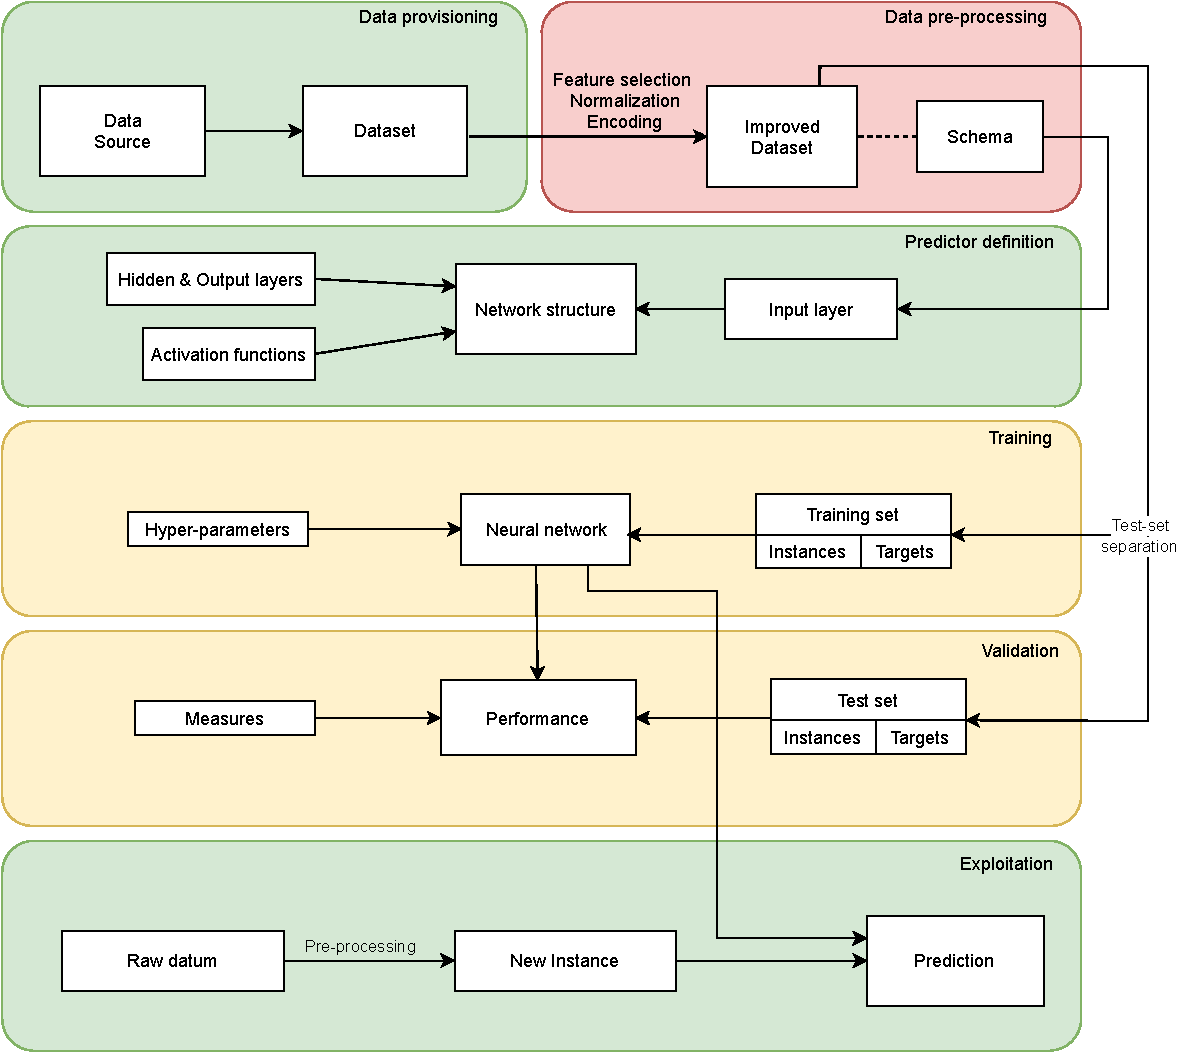
\includegraphics[width=.7\linewidth]{figures/phases1.pdf}
    \end{center}

\end{frame}
%\\\\\\\\\\\\\\\\\\\\\

\subsection{The \twopkt{} Logic Ecosystem}

\begin{frame}{Overview}
    \begin{block}{The \twopkt{} project \hfill (\url{https://github.com/tuProlog/2p-kt})}
        \begin{itemize}
            \item Kotlin-based implementation of a logic ecosystem
            \item multi-platform, multi-OS, multi-paradigm
        \end{itemize}
    \end{block} 

    \begin{center}
        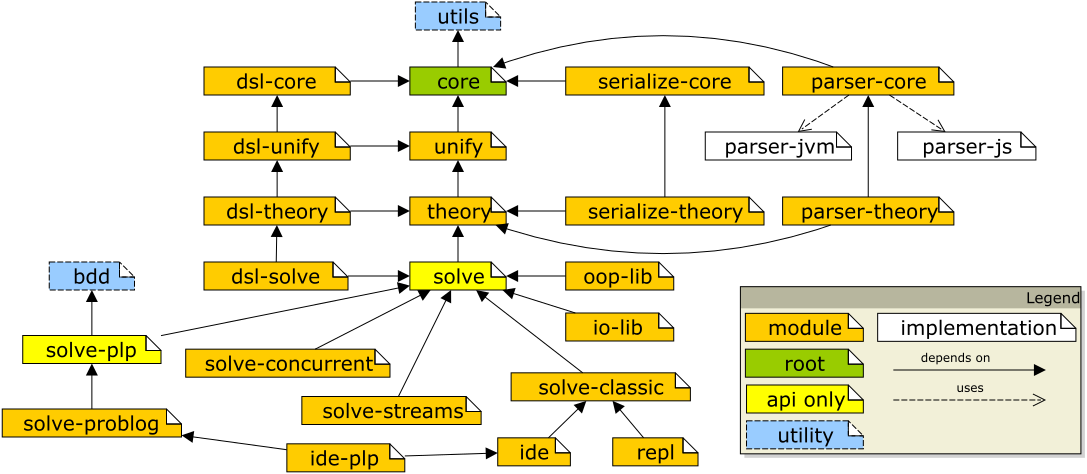
\includegraphics[width=.7\linewidth]{figures/project-map.png}    
    \end{center}

    \vspace{-.5cm}

    \begin{multicols}{2}
        \begin{itemize}\small
            \item knowledge representation
            
            \item \ldots and storage
            
            \item \ldots and parsing/presentation

            \item Prolog-like inference support
            %
            \item \ldots or concurrent / probabilistic
            
            \item LP--OOP interoperability
        \end{itemize}
    \end{multicols}
\end{frame}

\begin{frame}{\twopkt{}'s General API for Logic Resolution\ccite{2pkt-jelia2021}}

    \begin{columns}
        \begin{column}{.49\linewidth}
            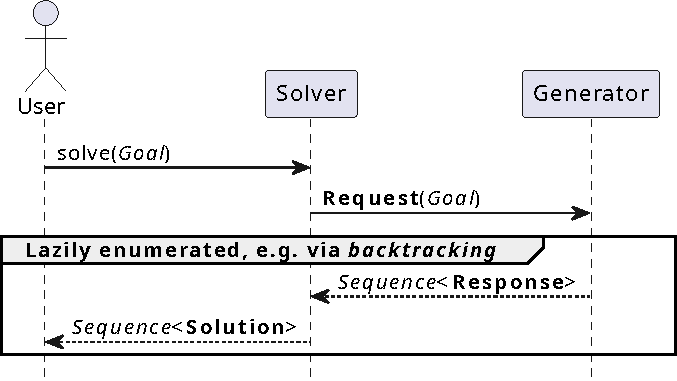
\includegraphics[width=\linewidth]{figures/primitive-usage.pdf}
        \end{column}
        \begin{column}{.49\linewidth}
            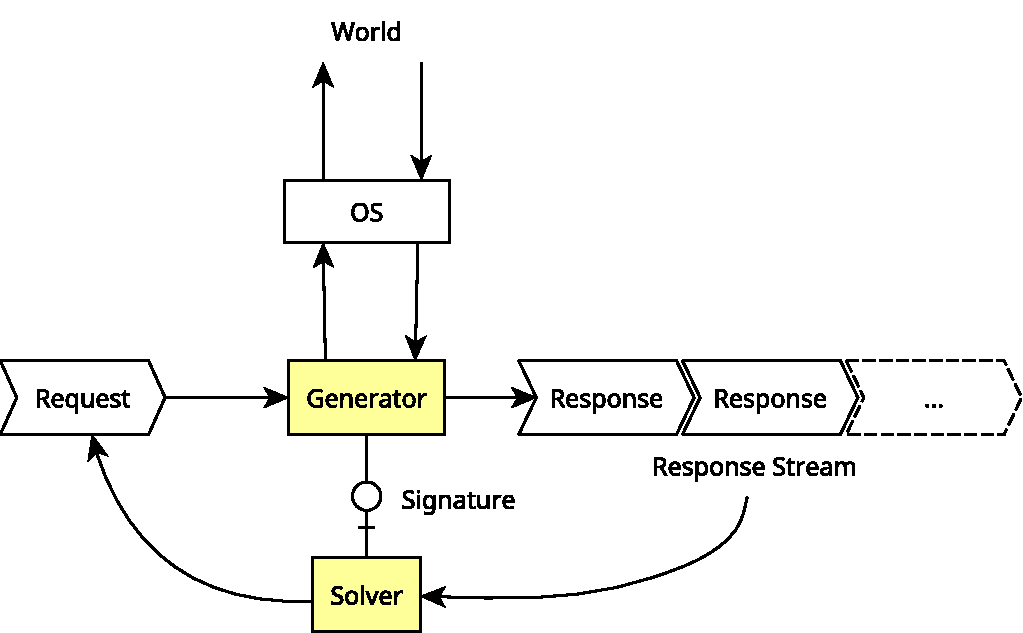
\includegraphics[width=\linewidth]{figures/generator.pdf}
        \end{column}
    \end{columns}

    \vfill

    \begin{itemize}
        \item Logic solvers as \alert{oracles} queried by users
        
        \vfill

        \item Generators as \alert{gateways} towards the external world
    \end{itemize}
\end{frame}

\section{Contributions}

\subsection{Expected benefits}

%\\\\\\\\\\\\\\\\\\\\\
\begin{frame}%[allowframebreaks]
\frametitle{Overview on expected benefits}

    \begin{itemize}
        \item Hybrid reasoning
    
        \item Declarative ML
    
        \item Symbolic data sources
    
        \item Model selection via resolution
    
    \end{itemize}

\end{frame}
%\\\\\\\\\\\\\\\\\\\\\

%\\\\\\\\\\\\\\\\\\\\\
\begin{frame}%[allowframebreaks]
    \frametitle{Hybrid reasoning}

    \begin{itemize}
        \item treating trained ML predictors as ordinary logic predicates
        \item hence enabling the combined exploitation of LP and ML
    \end{itemize}

    \prologimport{listings/hybrid-predictor.pl}

\end{frame}
%\\\\\\\\\\\\\\\\\\\\\

%\\\\\\\\\\\\\\\\\\\\\
\begin{frame}%[allowframebreaks]
    \frametitle{Declarative ML}

    \begin{itemize}
        \item use logic programs as declarative specification for ML aspects
    \end{itemize}

    \prologimport{listings/neural-network-declare.pl}

\end{frame}
%\\\\\\\\\\\\\\\\\\\\\

%\\\\\\\\\\\\\\\\\\\\\
\begin{frame}%[allowframebreaks]
    \frametitle{Symbolic data sources}

    \begin{itemize}
        \item use logic theories as datasets, and train predictors upon them
    \end{itemize}

    \prologimport{listings/logic-dataset-loading.pl}

\end{frame}
%\\\\\\\\\\\\\\\\\\\\\

\section{Conclusions \& future works}

%\\\\\\\\\\\\\\\\\\\\\
\begin{frame}%[allowframebreaks]
\frametitle{Conclusions \& future works}

\begin{block}{Summing up}
    Summarise the most relevant contributions of this study:
    %
    \begin{itemize}
        \item conclusion 1
        \item conclusion 2
        \item conclusion 3
    \end{itemize}
\end{block}

\begin{exampleblock}{Future works}
    Sketch some future research directions
    %
    \begin{itemize}
        \item future work 1
        \item future work 2
    \end{itemize}
\end{exampleblock}

(may be split into 2 slides)

\end{frame}
%\\\\\\\\\\\\\\\\\\\\\

%===============================================================================
\section*{}
%===============================================================================
\frame{\titlepage}

%===============================================================================
\section*{\bibname}
%===============================================================================

\setbeamertemplate{page number in head/foot}{}
%\\\\\\\\\\\\\\\\\\\\\
\begin{frame}[t,allowframebreaks,noframenumbering]\frametitle{\refname}
% \begin{frame}[c]\frametitle{\refname}
	\footnotesize
%	\scriptsize
    \bibliographystyle{apalike-AMS}
    % \bibliographystyle{plain}
	\bibliography{cilc-2022-logic-api-ml-talk}
\end{frame}
%\\\\\\\\\\\\\\\\\\\\\

%%%%%%%%%%%%%%%%%%%%%%%%%%%%%%%%%%%%%%%%%%%%%%%%%%%%%%%%%%%%%%%%%%%%%%%%%%%%%%%%
\end{document}
%%%%%%%%%%%%%%%%%%%%%%%%%%%%%%%%%%%%%%%%%%%%%%%%%%%%%%%%%%%%%%%%%%%%%%%%%%%%%%%%
